\newpage
\section{Shape database}
\label{sec:shapedatabase}
All physical objects within a simulation are \emph{shapes}. For example the following things are all shapes; a layer of a solar cell; a layer of an OLED; a lens; a complex photonic crystal structure; contact stripe on an OFET; the complex hexagonal contact on a large area device (see figure \ref{fig:alldevices} for more examples). These \emph{shapes} are defined using triangular meshes for example a box which is used to define layers of solar cells, and layers of LEDs is defined using 12 triangles, two for each side.  This box structure can be seen in figure \ref{fig:shape_box}.

\begin{figure}[H]
\centering
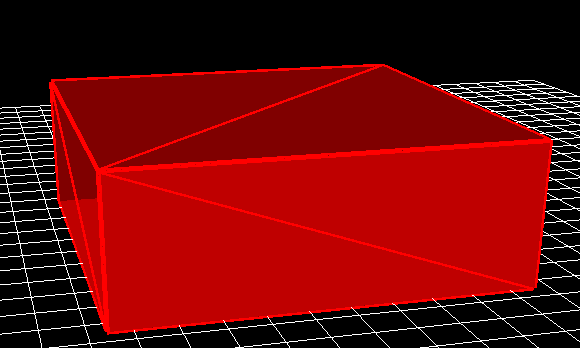
\includegraphics[width=0.5\textwidth]{./images/database_shapes/box.png}
\caption{the box \emph{shape}.}
\label{fig:shape_box}
\end{figure}

Shapes are stored in the shape database, this can be accessed via the database ribbon and clicking on the Shapes icon, see figure \ref{fig:shapedb}. By clicking on the \emph{shape database} icon the shape database window can be brought up see figure \ref{fig:shapedb_window}.

\begin{figure}[H]
\centering
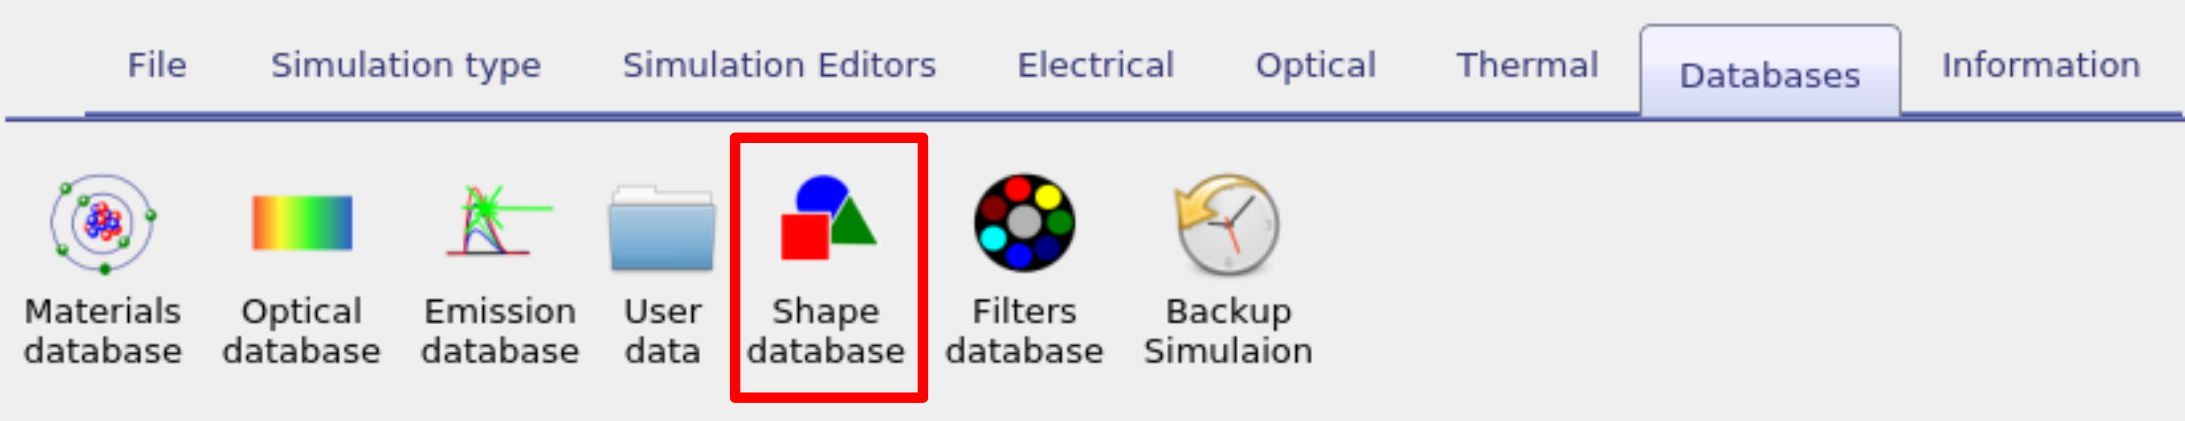
\includegraphics[width=0.8\textwidth]{./images/database_shapes/database_shapes.png}
\caption{Opening the shape database}
\label{fig:shapedb}
\end{figure}

\begin{figure}[H]
\centering
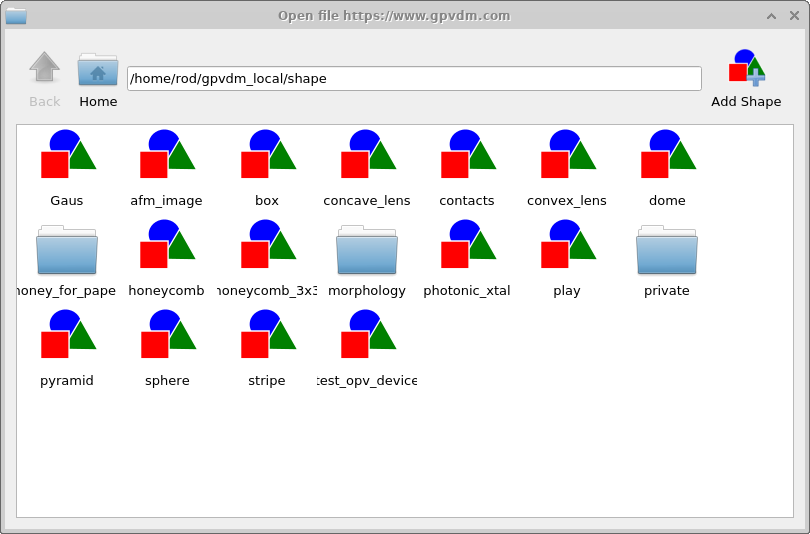
\includegraphics[width=0.8\textwidth]{./images/database_shapes/shape_db_window.png}
\caption{The shape database window}
\label{fig:shapedb_window}
\end{figure}

Try opening some of the shapes and have a look at them.  You will get a window much like that shown in figure \ref{fig:shapedb_example}. Figure \ref{fig:shapedb_example} shows a honeycomb contact structure of a solar cell.  On the left of the window is the 3D shape, and on the right of the window is the 2D image which was used to generate it.  Overlaid on the 2D image is a zx projection of the 3D mesh. The process of generating a shape involves first defining a 2D png image which you want to turn into a shape, in this case the 2D image is a series of hexagons and a bar at the top.  This image is then converted into a triangular mesh using a discretization algorithm.    

\begin{figure}[H]
\centering
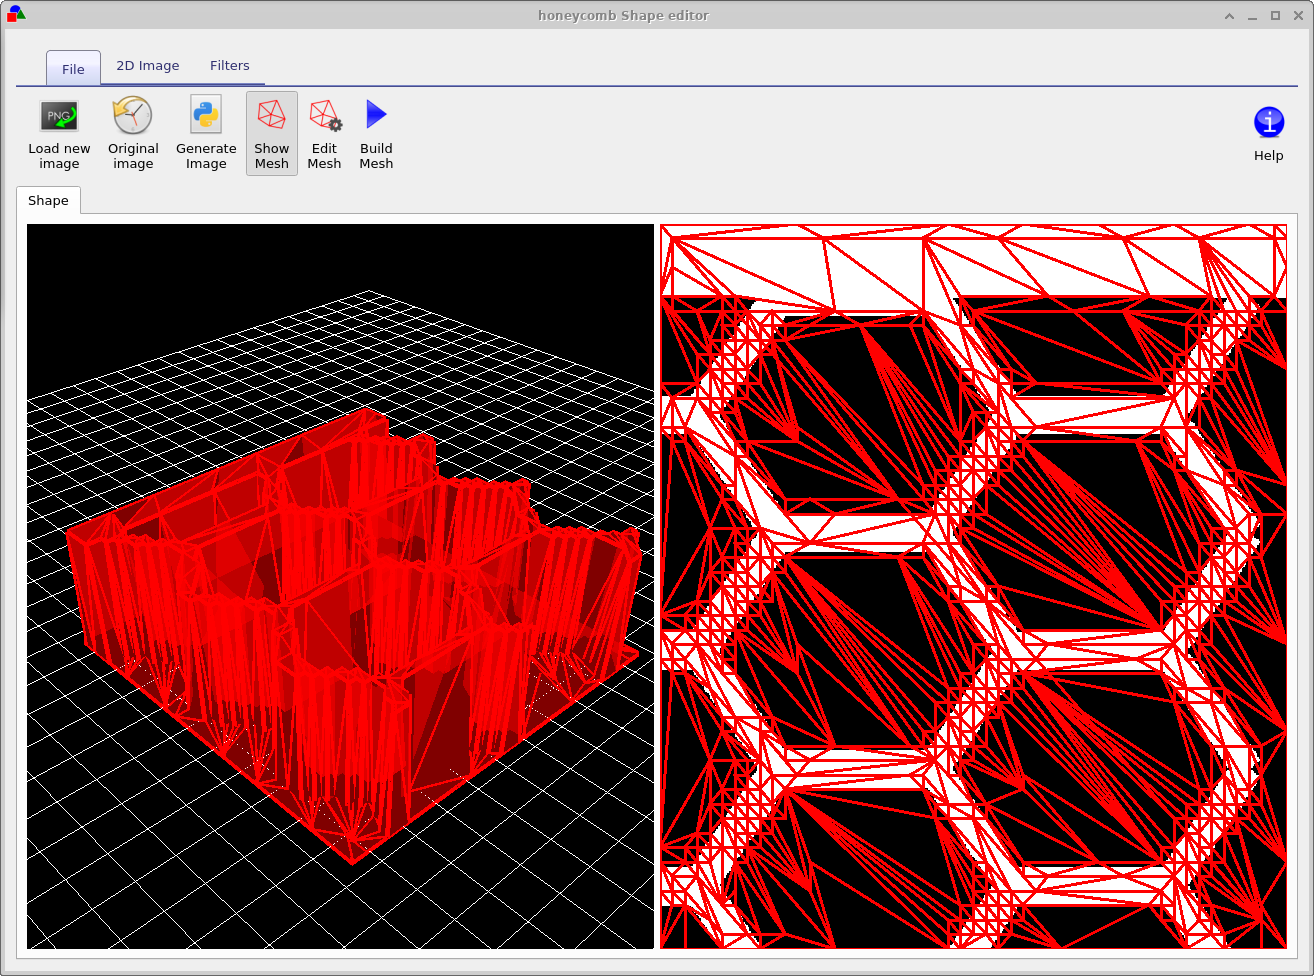
\includegraphics[width=0.7\textwidth,height=0.4\textheight]{./images/database_shapes/shape_db.png}
\caption{An example of a shape generated from a 2D png image. The 3D shape representing a hexagonal contact from a solar cell is on the left of the figure while the original 2D image is on the right.}
\label{fig:shapedb_example}
\end{figure}

Now try opening the shape \emph{morphology/1} and you should see a window such as the one shown in figure \ref{fig:shape_examples01}, in the file ribbon find the icon which says \emph{show mesh}.  Try toggling it of and on, you will see the 2D mesh become hidden and then visible again.  This example is a simulated bulk heterojunction morphology, but you can turn any 2D image into a shape by using the \emph{load new image} button in the file ribbon.  Try opening the mesh editor by clicking on \emph{Edit Mesh} the \emph{file} ribbon, you should get a window looking like figure \ref{fig:shapedb_config_window}. This configure window has three main options \emph{x-triangles}, \emph{y-triangles} and \emph{method}.  The values in \emph{x-triangles}, \emph{y-triangles} determine the maximum number of triangles used to discretize the image on the x and y axis.  Try reducing the numbers to 40 then click on \emph{Build mesh} in the file ribbon.

\begin{figure}[H]
\centering
\begin{tabular}{ c c }

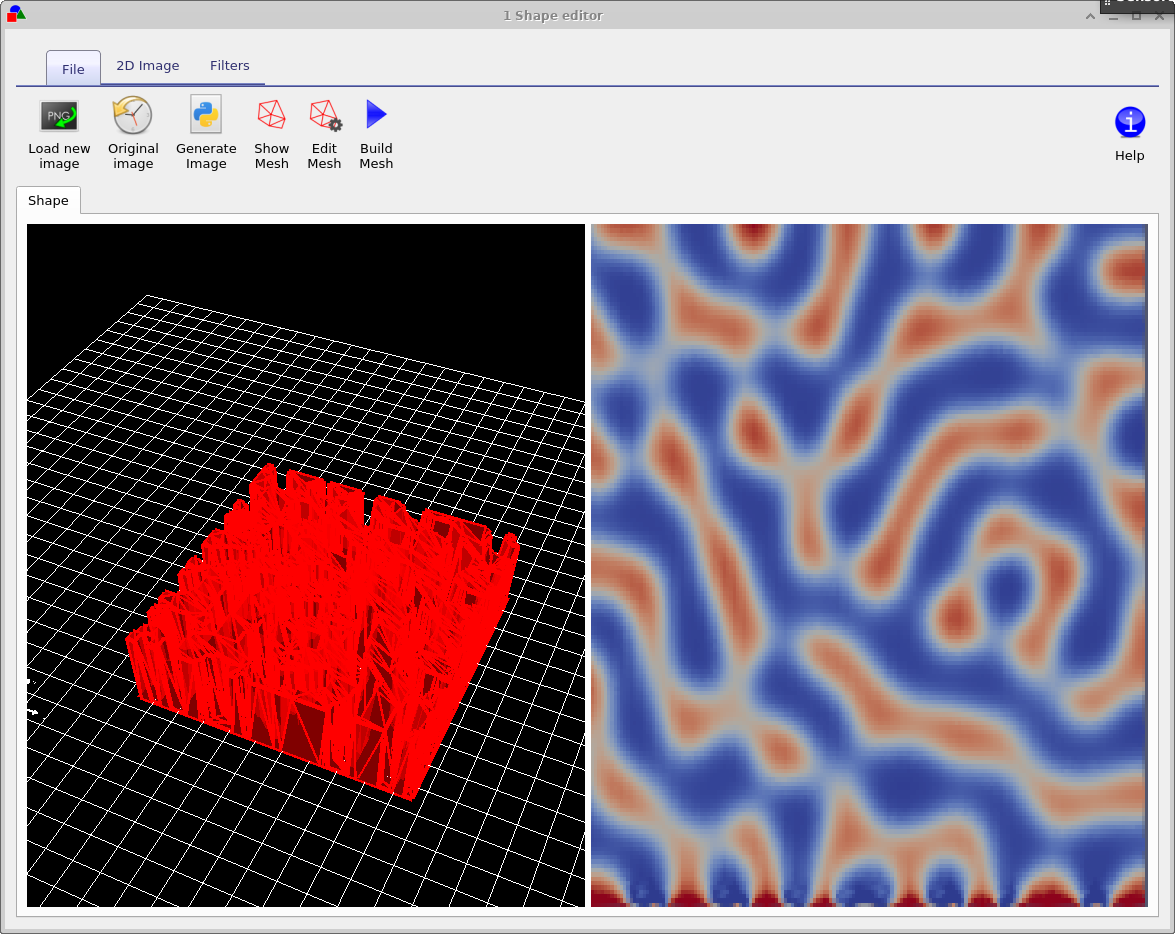
\includegraphics[width=0.5\textwidth,height=0.4\textwidth]{./images/database_shapes/example0.png}

&
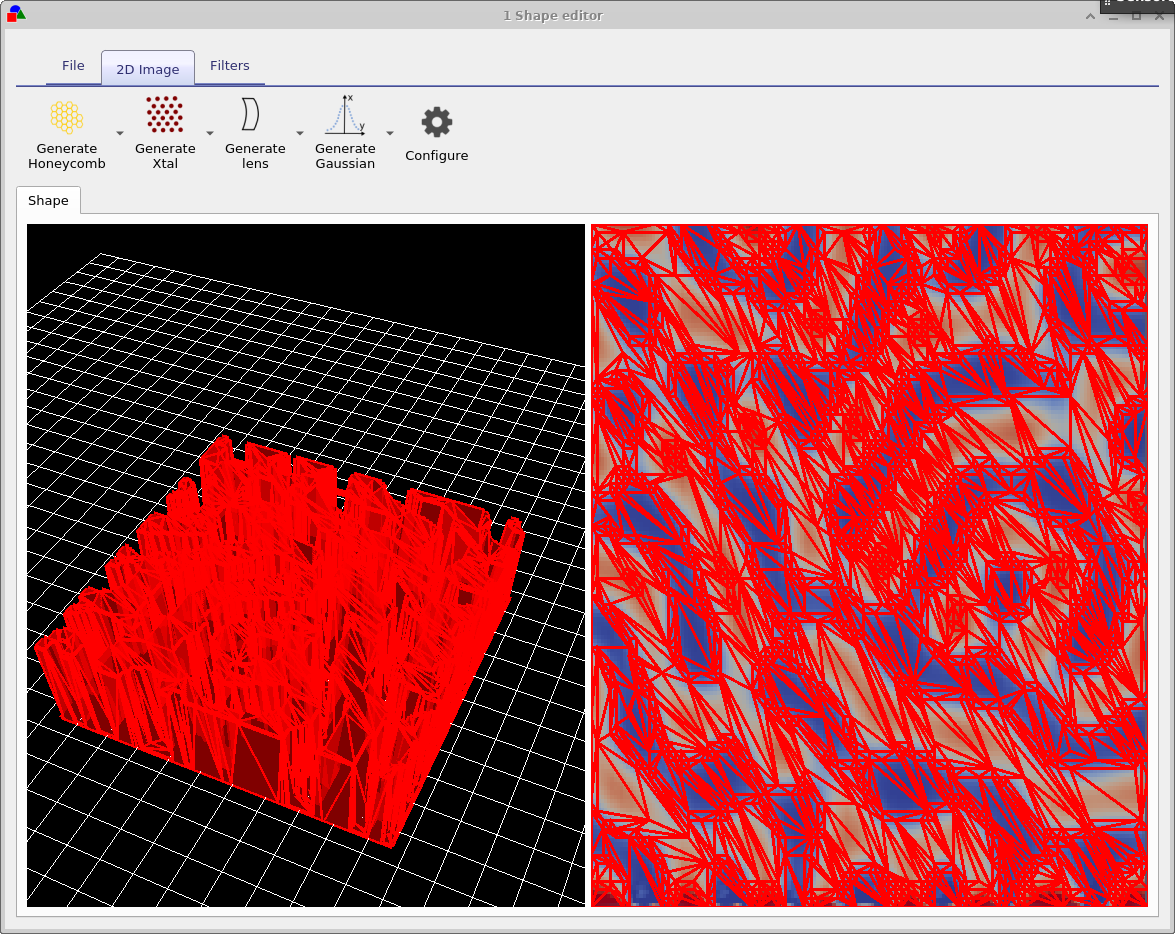
\includegraphics[width=0.5\textwidth,height=0.4\textwidth]{./images/database_shapes/example1.png}
\\
\end{tabular}
\caption{Clockwise from the top left; The imported absorption sepctrum; The basic material parameters; The electrical parameters; and the Thermal parameters.}
\label{fig:shape_examples01}
\end{figure}

You will see that the number of triangles used to describe the image reduce.  The more triangles that are used to describe the shape the more accurately the shape can be reproduced, however the more triangles are used the more memory a shape will take up and the slower simulations will run.  There is always a trade off between number of triangles used to discretize a shape. Try going back to the \emph{Edit Mesh} window and set \emph{method} to \emph{no reduce} and then click on \emph{Build mesh} from the file menu again.  You will see that the complex triangular mesh as been replaced by a periodic triangular mesh, which is more accurate but requires the full 70x70 triangles.  The difference between the \emph{no reduce} and \emph{Node reduce} options are that \emph{no reduce} simply uses a regular mesh to describe and object and \emph{Node reduce} starts off with a regular mesh then uses a node reduction algorithm to minimize the number of triangles used in the mesh.

\begin{figure}[H]
\centering
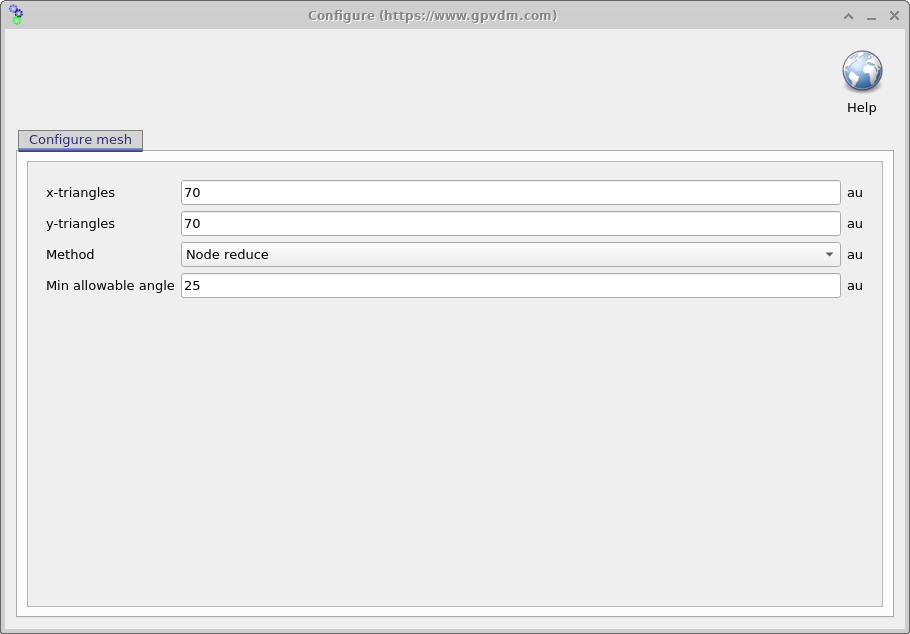
\includegraphics[width=0.7\textwidth]{./images/database_shapes/config_window.png}
\caption{The mesh editor window, accessed via the file ribbon.}
\label{fig:shapedb_config_window}
\end{figure}

As well as loading images from file, the shape editor can generate it's own images for standard objects used in science, the 2D image ribbon is visible in the right hand panel of figure \ref{fig:shape_examples01}.   There are options to generate lenses, honeycomb structures and photonic crystals. Each button has a drop down menu to the right of it which can be used to configure exactly what shape is generated.

The final ribbon to be discussed is the \emph{Filters} ribbon. This is used to change loaded images, try turning on and off the threshold function.  This applies a threshold to an image so that RGB values above a given value are set to white and those below are set to black.  There are also other functions such as Blur, and Boundary which can be used to blur and image and apply boundaries to an image.

\begin{figure}[H]
\centering
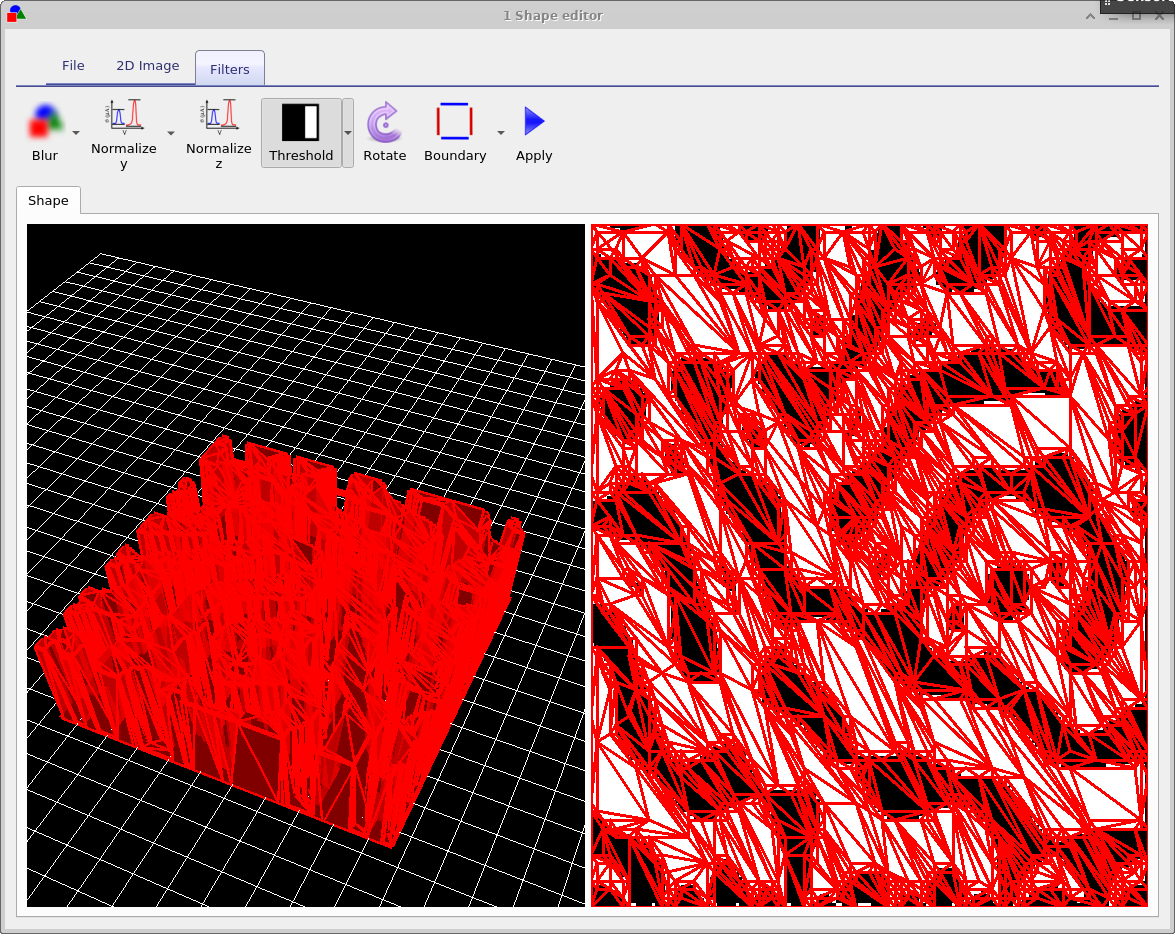
\includegraphics[width=0.7\textwidth]{./images/database_shapes/example2.png}
\caption{The shape database}
\label{fig:shapedb_example2}
\end{figure}


\subsection{The shape file format}

A shape has to be a fully enclosed volume, if you use the built in shape discretizer this will be done for you automaticity.  However if you are building shapes by hand you will have to enforce this condition. Each shape directory contains the following files

\begin{table}[H]
\begin{center}
\begin{tabular}{ |c|c|c| } 
 \hline
	File name 			& 	Description  \\ 
 \hline
	$data.json$ 			&	Holds the configuration for the shape file \\ 
	$image\_original.png$ 	&	backup of the imported image\\ 
	$image\_out.png$ 	& The final processed image  \\
	$image.png$ 	&	The imported image which may be modified.    \\
	$shape.inp$ 	&	The discretized 3D structure.   \\

 \hline
\end{tabular}
\caption{The files within a shape directory}
\label{tab:files_in_shape_dir}
\end{center}
\end{table}

The png files are of images in various states of modification.  The data.json file stores the configuration of the shape editor and the shape.inp file contains the 3D structure of the object.  An example of a shape.inp file is shown below in \ref{fig:shape_file_format}. The file format has been written so that gnuplot can open it using the splot command without any modification.  As such each triangle is comprised of four z,x,y points (lines 21-24), the first three lines define the triangle, and the forth line is a repeat of the first line so that gnuplot can plot the triangle nicely.  The number of triangles in the file is defined on line 18 using the \#y command.  The exact magnitudes of the z,x,y values do not matter because as soon as the shape is loaded all values are normalized so that the minimum point of the shape sits at 0,0,0 and the maximum point from the origin sits at 1,1,1.  When being inserted into a scene, the shape is then again renormalized to the desired size of the object in the device.


\begin{figure}[H]
\centering
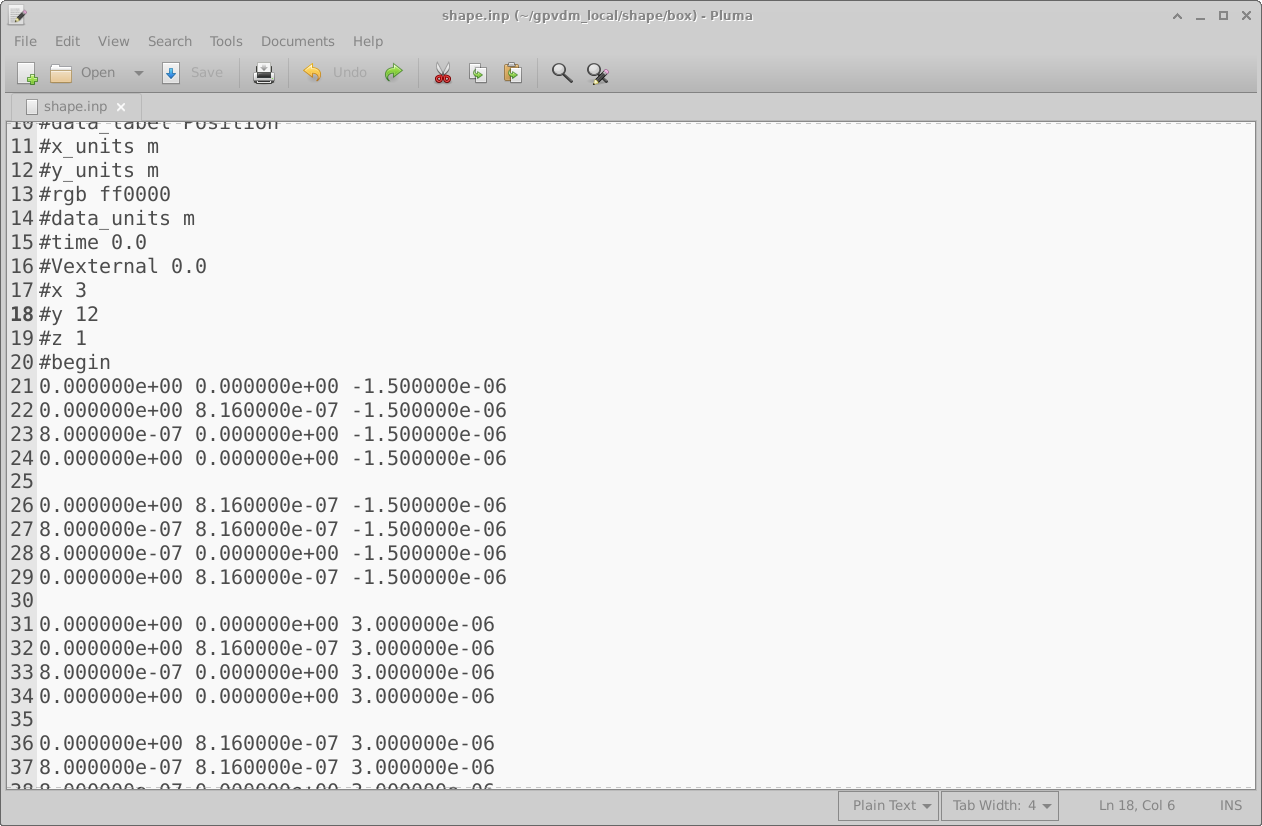
\includegraphics[width=0.7\textwidth,height=0.4\textheight]{./images/database_shapes/shape_file_format.png}
\caption{An example of the shape.inp file.}
\label{fig:shape_file_format}
\end{figure}



